\section{Background}
\label{S:tBack}
This section provides an overview of the research studies on pedestrian crossing behaviour, emphasizing trajectory prediction studies. Traditional approaches to pedestrian trajectory modelling and recent data-driven trends are discussed in this chapter. Modern data-driven approaches require novel large-scale datasets. In order to understand pedestrian behaviour in the presence of AVs, real datasets from AV manufacturers are the most reliable resources. Thus, a review of the available datasets from a pedestrian-oriented point-of-view is provided, followed by a discussion on data alternatives for AV-pedestrian studies.      
\subsection{Pedestrian trajectory prediction}
Early models in the literature tried to model the pedestrian movement using the concepts and theories of ideal gases~\cite{henderson1974fluid} or fluids~\cite{helbing1998fluid}. However, the turning point in pedestrian movement modelling was the social force model by Helbing and Molnar in 1995~\cite{helbing1995social}. Based on the idea that behavioural changes are caused by so-called social fields, Helbing and Molnar described forces affecting pedestrian behaviour as a result of internal motivations of an individual to decide and perform actions. In 2004, Antonini~\textit{et al.} applied logit-type discrete choice models to pedestrian movement analysis using video data~\cite{antonini2004simulation}. The microscopic approach of the model allowed a detailed analysis of pedestrian movement. The choices that a pedestrian was facing at a certain time in their model were: (1) speed level and (2) discrete radial direction. Utility functions for each of these choices were defined based on the presence of obstacles, proximity to the destination and positions and speeds of other pedestrians. Later works on these models added other variables, helping the model gain strength by of observing various factors. For instance, Guo \textit{et al.}~\cite{guo2012route} added visibility parameters to the model while Asano~\textit{et al.}~\cite{asano2010microscopic} later incorporated density. The major weaknesses of such microscopic methods using logit formulation is their requirement to discretize the space and speed into arbitrary levels. Furthermore, they are very myopic as they can only predict the next-step decision based on current conditions without incorporating what is ahead, e.g., approaching vehicle or a wall a few metres ahead.

The widespread success of machine learning methods in recent years, as well as the availability of large pedestrian datasets, have resulted in a shift of pedestrian research trends to data-driven. In particular, recurrent networks, i.e., RNN and LSTM, have been the dominant machine learning methods for trajectory prediction. In most cases, the input data used for trajectory prediction is only the past trajectory of the pedestrians~\cite{xue2019location,zhang2019sr,alahi2016social,gupta2018social}. In one of the significant earlier studies in the field, Alahi~\textit{et al.}~\cite{alahi2016social} introduced Social LSTM, a method that incorporated interactions among pedestrians in sequential models, namely Long Short-Term Memory (LSTM), to forecast trajectory of pedestrians using video footage of walking individuals in crowded scenes. In their method, a \textit{Social Pooling Layer} is added to the framework. Through this layer, LSTM layers trained for individuals in a scene share their information. In spite of the success of the Social-LSTM model in forecasting pedestrian trajectory, this model does not account for the contextual information on the environment and aspects like where the pedestrian is looking. The model may be applicable in pedestrian-dominant environments, e.g., shopping mall or train station, but is difficult to apply to situations like road crossing behaviours of pedestrians in an automated environment. Furthermore, the future trajectory predicted by Social-LSTM assumes a fixed-length future trajectory.  More recently, Gupta~\textit{et al.}~\cite{gupta2018social} introduced \textit{Social-GAN}, a model that predicts socially acceptable trajectories by training adversarial against a recurrent discriminator. Similar to~\cite{alahi2016social}, this model fails to capture context information from the environment, and its applicability is limited.

Some other research studies have incorporated contextual and semantic information into the pedestrian trajectory to predict their next locations~\cite{lee2017desire,chandra2019traphic,rasouli2019pie}. The semantic information used can be road design~\cite{bi2019joint}, the shape of objects~\cite{chandra2019traphic}, and the speed of the vehicles~\cite{bhattacharyya2018long,rasouli2019pie}. Lee~\textit{et al.}, for instance, added semantic contexts, such as road structure and interactions and dynamics of the agents to their proposed RNN model and predicted pedestrian trajectory of variable lengths in a video dataset~\cite{lee2017desire}. Despite all the diversity in models, data and objective functions in the relevant research studies, only a few models have attempted to predict pedestrian trajectory in the context of AVs. In most such cases, analyzing pedestrian is limited to crowds, and not in the context of interactions with vehicular traffic. To the best of our knowledge, almost all the models in the literature have used general-purpose video footage of pedestrian movements as the input data. Because pedestrian road crossing behaviour in the presence of AVs may differ, current datasets and scenarios may not apply to the futuristic scenarios. One of the reasons behind this gap can be traced back to the lack of pedestrian data in open-access AV datasets. In the next subsection, an overview of these datasets is provided.

\subsection{Open-Access AV datasets}
Despite the significant improvements in AVs' general operations through video and sensor datasets, pedestrian-AV interaction modelling using such datasets has not been thoroughly explored. AV datasets have been widely explored for object detection~\cite{chang2019argoverse}, semantic segmentation~\cite{porzi2019seamless}, and vehicle trajectory prediction~\cite{gu2020lstm,chandra2020forecasting,lee2017desire}. However, a lack of pedestrian behavioural studies using these open-access AV datasets made us explore the gaps and missing components in these datasets. In the rest of this subsection, an overview of four available open-access automated datasets is provided from a pedestrian-oriented point-of-view. 
\subsubsection{NuScenes}
With 1,000 scenes of 20 seconds each~\cite{nuscenes2019}, nuScenes is one of the largest open-access dataset available for AV research. The vehicle containing sensors (ego vehicle) in nuScenes' data collections is equipped with 6 cameras, 1 LIDAR\footnote{Light Detection and Ranging sensor} and 5 RADAR, GPS, and IMU\footnote{Inertial Measurement Unit sensors} sensors as the entire sensor suite of an AV. With around 5.5 hours of driving in congested urban areas of Boston and Singapore, nuScenes is a suitable match for studying modern urban spaces. Twenty-three classes of objects are annotated in the dataset, including pedestrians, children, bicycles, construction zones, etc. High-quality annotations of pedestrians make it easier to extract relevant frames from the dataset and focus on the pedestrian side of the scenes. With detailed information on the ego vehicle position, the dataset enables finding the vehicle-to-pedestrian distance at each time frame. Although the dataset is inclusive in different weather conditions, vegetation, and road markings, such information is not provided in the dataset and needs to be extracted by processing frames and videos. Including the underlying maps of the ego vehicle is another advantage that the nuScenes dataset provides, enabling extracting some context from the map. \cref{fig:nusc} shows a sample image from different cameras of a nuScenes ego vehicle.
\begin{figure}
    \centering
    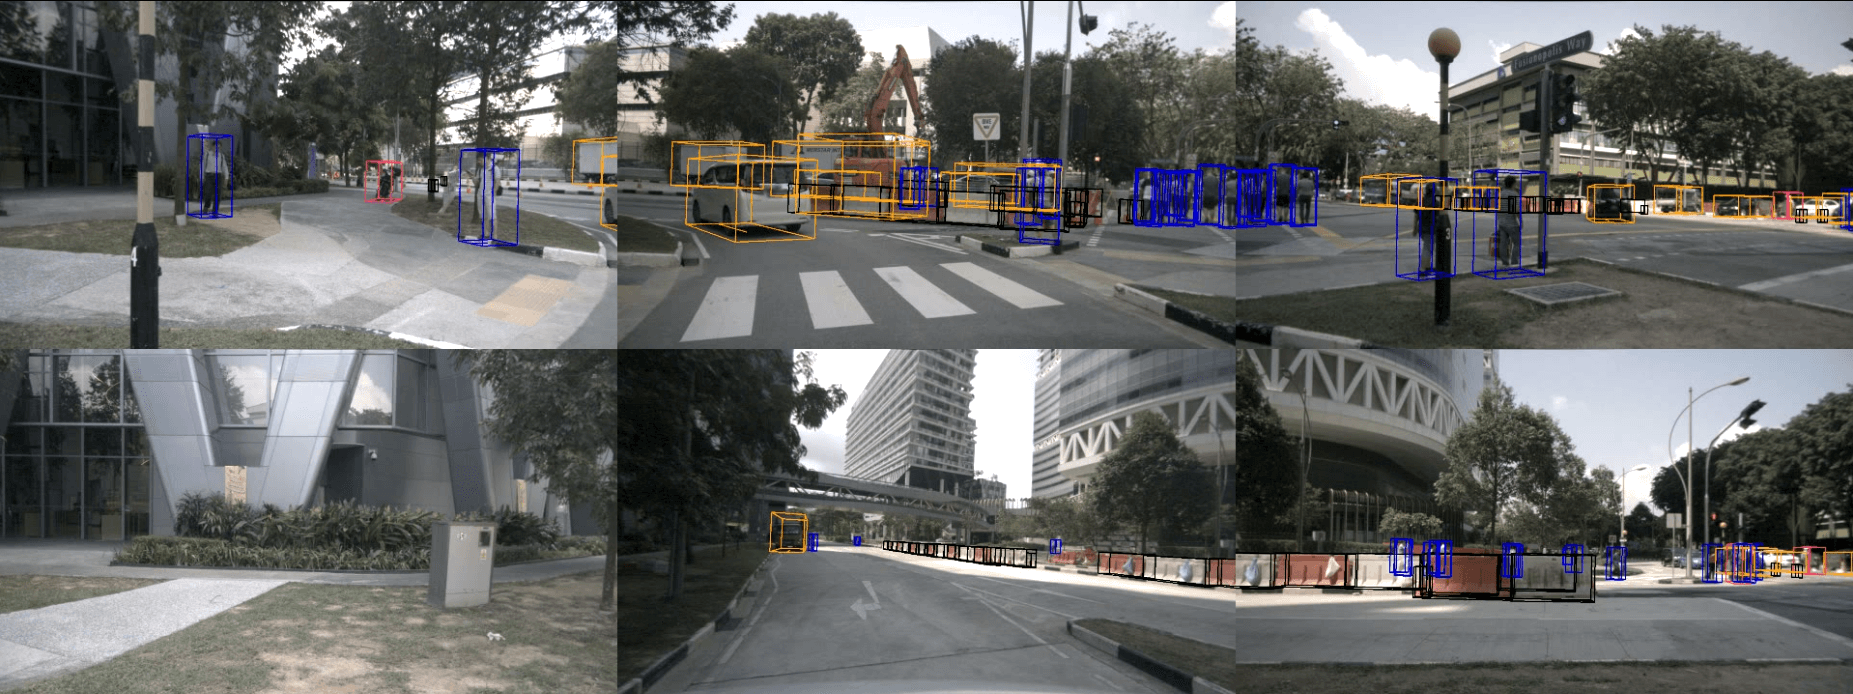
\includegraphics[scale=0.2]{chapter_6/figures/nusc.png}
    \caption{Object annotation example in nuScenes dataset (photo from \href{https://www.nuscenes.org/}{nuScenes})}
    \label{fig:nusc}
\end{figure}

\subsubsection{Lyft Level 5 open data}
Built upon the nuScenes database schema, Lyft level 5 dataset provides 2.5 hours of automated driving in Palo Alto, California~\cite{lyft2019}. Similar to nuScenes, underlying maps, annotations and different weather conditions are included in the dataset. Although it is relatively new, using the same database format as nuScenes gives Lyft level 5 dataset a robust and well-documented structure.  
\cref{fig:lyft} depicts a schematic image of a Lyft automated vehicle and its sensors.
\begin{figure}
    \centering
    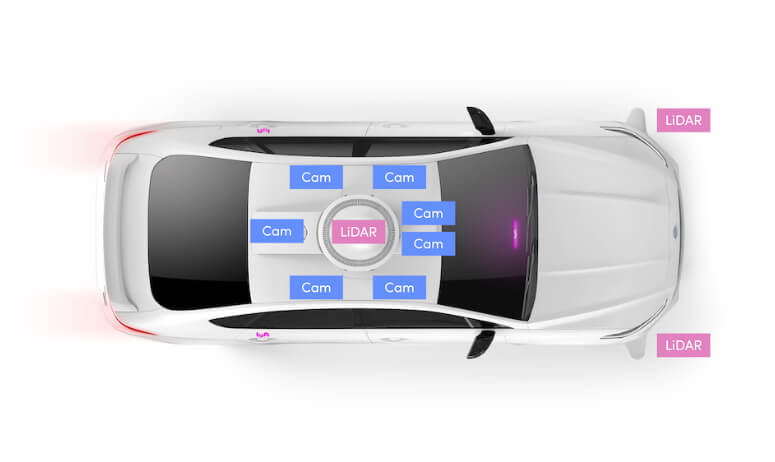
\includegraphics[scale=0.5]{chapter_6/figures/lyft.jpg}
    \caption{A schematic representation of a Lyft ego vehicle with all its sensors locations (photo from \href{https://self-driving.lyft.com/level5}{Lyft})}
    \label{fig:lyft}
\end{figure}  
\subsubsection{Waymo}
As of November 2020, Google's Waymo dataset is the largest and most annotated AV data available~\cite{sun2020scalability}. With  1150 scenes of over 6 hours of driving, the covered 76 $km^2$ area in the Waymo dataset is the largest among all the available datasets. Using three coordinate systems and providing means to transform data between frames, it is easy to follow and extract the trajectories of objects by having the positions of objects both in global coordinates and vehicle frame (relative to the ego vehicle position). Extensive hours of data collection include driving in various scenarios, including night time and daylight, construction areas, downtown and suburban areas, and diverse weather conditions. The recordings have been captured in Phoenix, Mountain View and San Francisco, enabling research opportunities in domain adaptations. The database format used for Waymo is new and different from those of other datasets, making the application of the models designed based on other datasets require further data cleaning procedures. However, having an active GitHub community with strong documentation helps smooth this transition. Unlike other popular AV datasets, the Waymo dataset currently does not include an underlying map of the events, making utilization of semantic information of the map in the algorithms impossible.   
\cref{fig:waymo} shows an annotated LIDAR data sample from Waymo dataset.
\begin{figure}
    \centering
    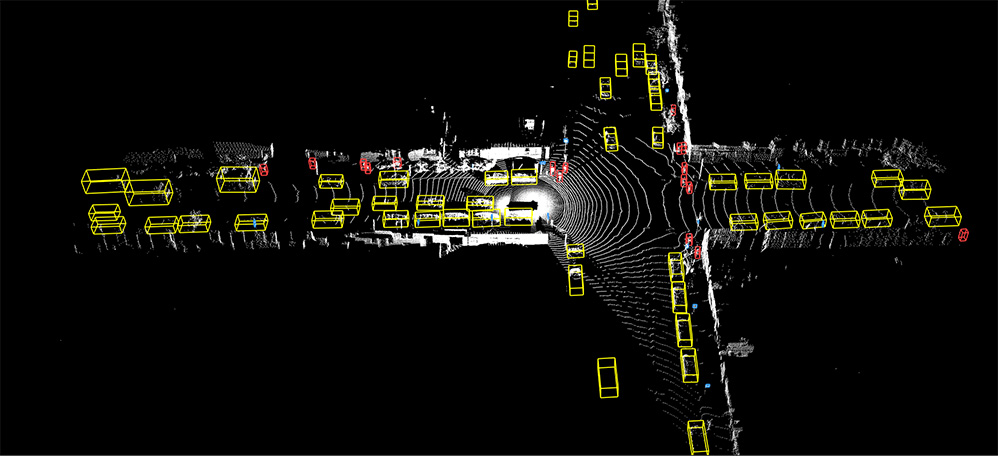
\includegraphics[scale=0.4]{chapter_6/figures/waymo.jpg}
    \caption{An annotated LIDAR data sample (photo from \href{https://waymo.com/open/data/}{Waymo})}
    \label{fig:waymo}
\end{figure}    

To study unsignalized crossing behaviour of pedestrians, we investigated NuScenes, Waymo and Lyft level 5 datasets to extract the relevant frames to the objective of this study.

\subsubsection{Pedestrian crossing in AV datasets}
We extracted pedestrian instances based on the LIDAR data of Lyft, nuScenes and Waymo dataset, and the annotations provided. We defined seven criteria and applied them to the datasets to narrow down to events involving mid-block crossings of pedestrians. The defined criteria are:
\begin{enumerate}
    \item Pedestrian is detected in front of the car: as LIDAR data enables detection of pedestrians even if they are on the rear side, a proportion of pedestrians detected are not interacting with the ego vehicle when during the scene. This filter makes sure that the ego vehicle is or will interact with the pedestrian during the scene
    \item Pedestrian is seen on both left and right sides of the ego vehicle: to limit the event to pedestrian crossings, it is expected that during the scene, the pedestrian is detected on both sides of the ego vehicle
    \item Pedestrian is moving in front of the ego vehicle: remove instances of pedestrians waiting, waling on the sidewalk, sitting, etc.
    \item Trajectory of detected pedestrians form an angle of 45 to 135 degrees with the trajectory of the ego vehicle
    \item Ego vehicle's change of direction forms an angle of less than 60 degrees. This filter is added to avoid turning vehicles to be included as they might pass all the previous criteria with no crossing of pedestrian taking place
    \item The distance between a pedestrian and the ego vehicle is less than 50 meters
    \item Pedestrian and ego vehicle have intersecting trajectories meaning that they path a similar point during the scene
\end{enumerate}
It should be noted that due to the short length of scenes, the last criteria should be loosened as ego vehicle might not necessarily pass the points that pedestrian is observed. The scenes related to remained data are then manually observed to verify if a pedestrian is crossing mid-block in front of the ego vehicle.

We start with the Lyft dataset, as the smallest dataset of all. In total, 350 scenes were available within the original dataset. Not considering the distance, and applying the first five filters, 137 possible instances of jaywalking pedestrians are found. However, when the instances are limited to a 50-meter maximum distance between pedestrian and ego vehicle, only 20 instances remain. After carefully watching the 20 remained instances, it appeared that no jaywalking events occurred within the dataset. The relatively short 2.5 hours length of the Lyft dataset can be mentioned as the reason behind the failure to find any instances. 

Moving forward to nuScenes dataset with the same format as Lyft level 5, 5.5 hours of driving is available in nuScenes dataset, leading to a compressed size of 350 GB. After tracking and detecting pedestrians among different frames of scenes using annotation IDs, 8,143 unique pedestrians were found and tracked in the dataset. After applying all the criteria defined, 200 of the instances remain in the dataset. However, by viewing the videos of the remaining instances, it appears that further filters are required in order to extract jaywalking instances more accurately. For example, in some instances the ego vehicle is interacting with a pedestrian in a parking lot or a private driveway. Although such instances meet the criteria define in our filters, they cannot be categorized as mid-block crossing events. Having more information about the environment that the ego vehicle is driving can help distinguish such instances automatically without the need for manual subjective observations or complex video processing. 

Finally, the Waymo dataset was investigated to extract crossing pedestrian events. In the first step, an impressive number of 23,056 unique pedestrians were tracked between the frames. However, only 1,182 of the total pedestrians passed filter 1 and were detected in front of the car. By applying filter 2, 280 of the remaining pedestrians passed the criteria of being observed on both sides of the ego vehicle. One hundred of the remaining pedestrians were removed from the data by adding the walking filter, leading to 211 instances of potential mid-block crossings. By applying the angle criteria, 117 pedestrians were left in the dataset. However, when observing the video data of the remaining instances, it appeared that a major part of the crosses was related to ego vehicle turning events, which made the walking pedestrians on the sidewalks pass all the previous filters. By introducing filter 5 and focusing on vehicles following a relatively straight trajectory, only 55 instances were left in the dataset.

By investigating some of the most well-established open-access AV datasets it appears that in order to extract events of a specific behaviour of pedestrians, larger and more extensive datasets are required. A solution to overcome this challenge would be to combine data from different resources to create a hybrid dataset focused on pedestrians. However, difference in data formats, sensors, environments and coordinate systems used make it a challenging and difficult task to combine these datasets. Another solution would be to collect data with a particular focus on pedestrians. However, most popular video datasets used for pedestrian behaviour analysis are dedicated to pedestrian interactions with each other and their dynamics in crowds~\citep{robicquet2016learning,zhang2019widerperson}. In recent years, some researchers have tried to address this issue and collect and provide pedestrian-oriented AV datasets~\cite{dipietro1970pedestrian,kotseruba2016joint}. However, these datasets are still not well-established in the literature. To understand the most essential context information required for pedestrian trajectory studies, we develop a controlled virtual reality experiment. The controlled nature of our data allows us to record pedestrian behaviour under several customized conditions and test the effects of various contextual information on the model accuracy.     